\section{Základy}

V této části se podíváme na vstupní zarušený signál, který nám byl přiřazen a jeho vlastnosti.0
Vstupní signál je načten funkcí soundfile.read, která vrací pole samplů signálu jako numpy.arrray a vzorkovací frekvenci.
Signál byl vykreslen pomocí matplotlib.plot, pro hodnoty aplitudy byli použity přímo načtené hodnoty vzorků z předchozího kroku a časová osa byla vygenerována pomocí np.arange o velikosti počtu vzorků načteného signálu a vydělená vzorkovací frekvencí.

\begin{figure}[H] 
    \centering
    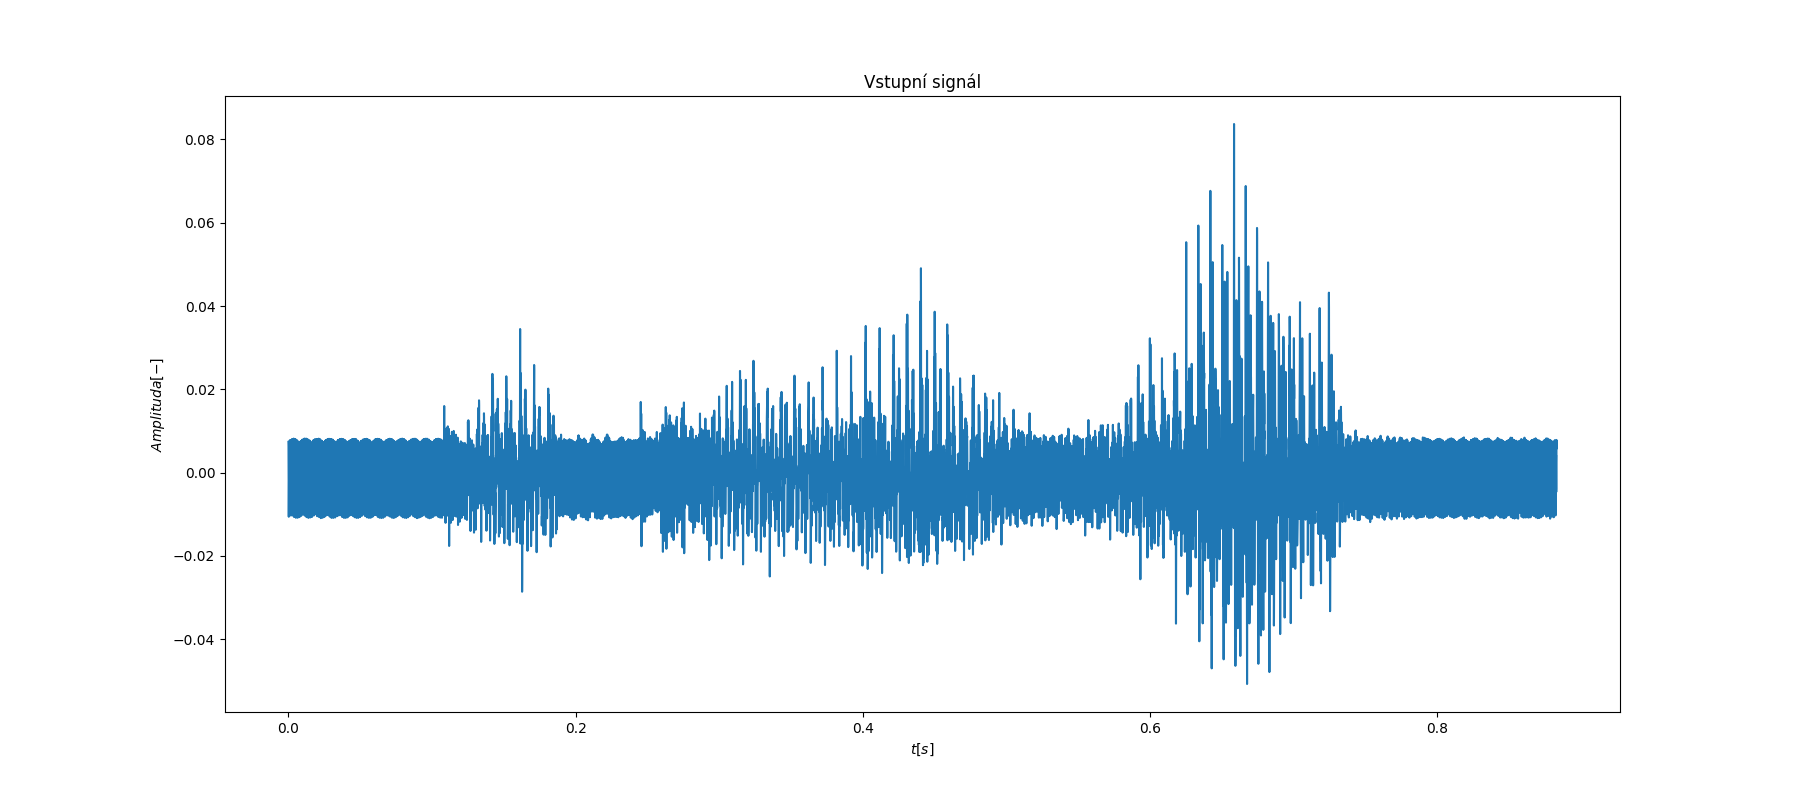
\includegraphics[scale=0.35,keepaspectratio]{Figure_1}
    \caption{Načtený signál}
\end{figure}

Délku signálu ve vzorkách lze získat přímo z pole vzorků a jeho hodnoty "size". Délka v sekundách byla získána vydělením délky ve vzorcích vzorkovací frekvencí.
Maximální a minimální hodnota byla získána pomocí buildin funkce pythonu "max" a "min".

Délka vstupního signálu je 14132 vzorků což při vzorkovací frekvenci 16kHz odpovádá 0.88325s.
Maximální hodnota tohoto signálu je přibližně 0.837097 a minimální přibližně -0.050751.
